%======================================================================
\chapter{Applications of Studying API Usage}
\label{sec:applications}
%======================================================================
In this chapter, we first present a classification framework for classifying API uses and also present a few API usage patterns. We then discuss two applications of our results from Chapter~\ref{sec:apiusage}. The first is the visualization tool VizAPI which uses the results of our static and dynamic analyses tool to create visualizations for developers to understand API usage in their components. The second is library fission, which we also perform using the results of our static and dynamic analyses tool.


\section{Classification of API Uses}
\label{sec:classification}

We now present a conceptual framework that outlines four dimensions along which a potential API use can be classified. We phrase the four dimensions as questions; each API usage has an answer for each of the questions. They are as follows: \emph{what}, \emph{how} \emph{which way} and \emph{why not}?

\begin{enumerate}
\item \emph{What} thing is being accessed?
\begin{itemize}
    \item types: user declares a subtype of a provider type;
    \item classes: user instantiates an object of a provider's class;
    \item annotations: user annotates a class or member with a provider-defined annotation;
    \item methods: user invokes a method from the provider; and,
    \item fields: user accesses a field defined in the provider.
\end{itemize}
\item \emph{How} is it accessed?
\begin{itemize}
    \item direct: user directly names thing being accessed;
    \item indirect: (methods only) thing being accessed differs from thing on declared type of the receiver object;
% we are using a runtime definition of virtual here: even if the call is declared virtual, we're calling it direct if declared target = actual target
    \item reflection/unsafe: user creates a handle to thing being accessed and uses that handle to perform the access;
% Mastrangelo says that, for our context, unsafe is used for serialization/deserialization, as sort of a super reflection.
    \item advanced dynamic: none of the above---user accesses thing in some other way, for example, via proxies.% or runtime code generation.
\end{itemize}
\item \emph{Which way} is the access going?
\begin{itemize}
    \item client user to library provider;
    \item library user to client provider, via callbacks.
\end{itemize}
\item \emph{Why not}, i.e. is the user bypassing access control?
\begin{itemize}
    \item access modifiers prevent the access, but are overridden;
    \item modularity conventions or mechanisms prevent the access: ``internal'' package, Java 9 modules, or OSGi;
    \item service loader restrictions prevent the access.
\end{itemize}
\end{enumerate}

The ``why not'' dimension differentiates uses from misuses; an API use that is allowed and expected by the API developer does not have an answer for ``why not''. Considering intended versus actual API surfaces gives another
perspective on the ``why not'' question. The other dimensions serve to classify the API use or misuse and understand which kinds of uses and misuses are most common. We intend for this framework to serve as a guideline for component developers who want to introspect about their software. Library developers can use this framework when they design new APIs to understand which parts of their library are most useful to clients and how. Client developers can use this framework to inspect how libraries are used and possibly to compare and contrast different libraries with the same functionality.

\section{API Usage Patterns}
\label{sec:patterns}

We now discuss API usage patterns with examples. Our examples use the \textit{connector-j} library\footnote{\url{https://github.com/mysql/mysql-connector-j/}, release 8.0.26}, which enables Java programs to communicate with MySQL databases. Namespaces are omitted for brevity. The standard Java library JDBC types belong to package \texttt{java.sql} and MySQL classes to packages \texttt{com.mysql.cj.jdbc.*}. Most of the code snippets are not considered best practice, and therefore illustrate API misuses.

We suggest that it is useful to think of misuse as on a
continuum rather than as a strict binary allowed-versus-not-allowed.
Some uses are more appropriate than others: when a
client passes an object to a serialization library, it is asking
the library to access even the private fields of that object, and so this
does not constitute a mis-use. Calling a deprecated API is less clear-cut.
Finally, explicitly calling into internal classes is likely to be a mis-use.
All bypasses some incur technical debt and add to the project's risk,
but some bypasses are more risky than others.


\subsection{Vanilla API Usage}

\lstdefinestyle{mystyle}{
	basicstyle=\ttfamily\footnotesize,
	breakatwhitespace=false,         
	breaklines=true,                 
	captionpos=b,                    
	keepspaces=true,                 
	numbers=left,                    
	numbersep=5pt,                  
	showspaces=false,                
	showstringspaces=false,
	showtabs=false,                  
	tabsize=2,
	frame = single
}

\lstset{style=mystyle}


MySQL JDBC driver class \texttt{com.mysql.cj.jdbc.Driver} implements the \texttt{java.\-sql.\-Driver} interface from the standard Java library. This is a case where the user, \textit{connector-j}, is a client of the standard library API. It is not bypassing any access control, directly accessing a \emph{type} from its library, and the access is going from the client to the library.

Shifting perspectives, \textit{connector-j} is intended for use as a library by its own clients. Its \texttt{Driver} implementation has a public constructor that can be \textit{directly instantiated} by its clients, as shown in line 1 of Listing~\ref{listing:direct-invocation}. It turns out that clients are not supposed to instantiate \texttt{Driver} classes themselves---JDBC documentation states that, for recent versions of JDBC, clients are supposed to call \texttt{DriverManager.getConnection()}. However, there are no compile-time or run-time checks prohibiting the instantiation of this object. We call this a \emph{modularity convention violation}. The part of the library that is being accessed is a class and the access is going from client (shown) to library (\texttt{connector-j}).  Although direct instantiation is not the intended use of the API, the library must provide a public constructor to enable service discovery.

Continuing with our example, line 2 of the same Listing~\ref{listing:direct-invocation} shows a \textit{direct invocation}. Although this call is a virtual method invoke, the declared type and actual types will always coincide in this example. There is no access control bypass here, and this is a direct invocation of a method call from the client to the library. We also observe \emph{indirect invocations}, i.e. virtual invokes where declared and actual differ.

%% In OO code, declared and actual types often differ, as seen at line 2 of Listing~\ref{listing:indirect-invocation}). The declared type is the interface \texttt{java.sql.Driver} while the actual type is class \texttt{com.mysql.cj.jdbc.Driver}. The only change between this \emph{indirect invocation} and the previous call is that the access is indirect, not direct. 

%The Java Virtual machine also includes the invokedynamic instruction to allow programmable method dispatch. The Java compiler occasionally generates this instruction, e.g. for dynamic code idioms like lambdas. There is no explicit receiver object for an invokedynamic and we do not consider such calls.

\lstinputlisting[language=Java,caption=Direct Instantiation and Invocation,label=listing:direct-invocation]{code-snippets/direct-invocation.java}

%% \lstinputlisting[language=Java,caption=Indirect Invocation,label=listing:indirect-invocation]{code-snippets/direct-virtual-invocation.java}

Our classification also allows for direct field accesses---from client to library or vice-versa (in the library to a client-provided parameter object). Of course, these may come with or without access control bypasses.

\subsection{Reflection and Reflective API Bypasses}
\label{ssec:api-usage-patterns:api-bypass}
Java reflection provides an alternate way for users to access APIs, i.e. it is an alternate ``how" something is accessed. Reflective accesses exist in practice and are more challenging to analyze statically than vanilla usages, as investigated by Landman et al~\cite{landman17:_chall_static_analy_java_reflec}; however, Bodden et al~\cite{bodden2011taming} have presented pragmatic workarounds based on recording dynamic information and using it statically. Clients request a reflective handle to classes, methods (and constructors), and fields, and call certain Java API methods to access the thing behind the handle. Listing~\ref{listing:reflection} shows a reflective instantiation of a \texttt{Driver}; prior to JDBC 4, this used to be the recommended way of creating a JDBC driver, but has been superceded by using a \texttt{DriverManager} to get a connection. We understand that this is not explicitly forbidden, but it is deprecated.

%% Instantiation, method invocation and field access is also possible through the reflection protocol in standard classes \texttt{Class}, \texttt{Method}, \texttt{Constructor} and \texttt{Field} in\texttt{ java.lang} and \texttt{java.lang.reflect}, respectively. We refer to these categories as \textit{INST-R}. \textit{INV-R }and \textit{FACC-R}, respectively. An example for reflective instantiation is shown in 

\lstinputlisting[language=Java,caption={Instantiating a \texttt{java.sql.Driver} via reflection},label=listing:reflection]{code-snippets/reflection.java}

Even if constructors, methods and fields and the classes declaring them are not visible, reflection can still be used to instantiate, invoke or access the respective things, subject to permission being granted by security managers. Listing~\ref{listing:reflection-private} shows the use of reflection to bypass access modifiers. While the class \texttt{ConnectionImpl} is public, the no-argument constructor has access modifier \texttt{protected}. However, reflection allows users to override access restrictions and call that constructor anyway. These are examples of a \textit{reflective API bypass pattern}. This call is thus a reflective-API-bypassing access to a constructor via reflection, from the client to the library. Line 3 makes the constructor accessible, using a pattern known as ``deep reflection''. Under Java 9, a user must provide a specific parameter to the JVM to allow such calls.

Java has mechanisms for preventing unwanted reflective accesses in general. In addition to preventing deep reflection and providing security managers, Java 9 also displays warnings about illegal reflective accesses to JDK internals. (Reflection can, of course, also be used to make calls that are part of a library's published API.)

\lstinputlisting[language=Java,caption=''Deep reflective'' instantiation bypassing visibility constraints,label=listing:reflection-private]{code-snippets/reflection-private.java}

% interesting but maybe not our point; I said things about it above.
%% Interestingly, prior to JDBC4, reflection was used to install a driver, consisting of the \texttt{Class.forName} call shown in line 1 of Listing~\ref{listing:reflection}. This triggered the execution of the static block of the respective class, leading to the instantiation and registration of the driver in  the JDBC  registry. 

%\todo[inline]{java 9 has illegal-reflective-access warnings which protects JDK internals from reflection. also they call it ``deep reflection'' when you use setAccessible to access private members. --add-opens allows this in java 9}

At this stage, we'd like to reiterate our goal in investigating API accesses. We've discussed vanilla API usages and reflective accesses to APIs. These two types of accesses have different affordances in terms of program evolution, and we aim to empirically evaluate how developers access libraries in practice, so that we (and others) can develop tools to help developers achieve more stability.

Upon a breaking upgrade, a vanilla API usage will fail to compile. Reflection is more dynamic---developers have the power to query the system and to adapt to the actual versions of the components that they are interacting with. If they use this power, then their code can be more resilient. However, failures that do arise can be more subtle and severe. The same phenomenon is present in Rinard's acceptability-oriented computing~\cite{rinard03:_accep}.

Dynamic techniques like reflection in data binding and persistence mapping pose additional perils. Even minor changes to classes can render data produced with previous versions un-readable. Adding, removing or modifying a field in a class mapped to a relational database table requires altering the table and migrating data. Adding a custom constructor (and thereby removing the default constructor) or removing a setter method may derail a deserialization mechanism based on the Java bean model (for example, \texttt{java.bean.XMLDecoder}). Binary serialization has long suffered from this problem. 

\subsection{Restricting API surfaces: Services, Package Names and Package Exports}
We mentioned that reflective instantiations of \texttt{Driver}s were recommended prior to JDBC 4. Post-JDBC 4, the recommendation is now to use the service loading mechanism to further reduce dependencies of clients on particular drivers. Specifically, the client is to use the \texttt{DriverManager} abstraction, which allows multiple drivers to bid on establishing a connection for a given database URL. (The client does not use the service loader directly.) 

\lstinputlisting[language=Java,caption={\tt Driver} instantiation through a service loader,label=listing:service-loader]{code-snippets/service-loader.java}

Service loading (described by Fowler in~\cite{fowler04:_inver_contr_contain_depen_injec}) is now widely used to register and access service implementations, for example, parsers, character sets, JDBC drivers, and JUnit5 extensions. 
Listing~\ref{listing:service-loader} shows an example of a client requesting an available \texttt{Driver} from a service loader (and not the {\tt DriverManager}) and using that driver to request a jdbc MySQL connection.
%Similar features for declarative services have been available for some time as part of OSGi~\footnote{OSGi services provide more features than Java service loading, including e.g. lifecycle management for services and the ability to wire, un- and rewire clients to the services they consume, but these are not relevant here.}. 

%Libraries advertise services as part of their metadata. This advertises both the capabilities of a component and its intended API. [Do we need this?]

Access modifiers are not the only way to protect APIs from being
called directly by clients.  Java's namespace is segregated by
hierarchical package names, but there are no enforced access controls
in plain Java. The Java standard library does state the modularity convention
that some of its implementation (specifically the classes living in
the \texttt{sun.*} namespace) is not to be used by clients, but this
convention is not enforced. Many libraries also use the convention that packages
named \texttt{internal} are not for use by clients. 

Java 
9 modules~\cite{corporation17:_java_platf_modul_system_jsr} and OSGi~\cite{alliance20:_osgi_core_releas_specif} offer other ways to delimit an intended API, in terms of a set of exported
packages. However, without enforcement, clients can use
all of the methods and fields of their libraries.

Enforcing the stated constraints requires additional support---either
a Java 9+ runtime or an OSGi container implementation. The Java 9+
compiler and runtime ensure that modules do not access modules to
which they do not have access, for example, non-exported modules. Under Java
9+, modules can also rely on having fine-grained control over
reflection permissions. Similarly, under an OSGi container implementation,
non-exported packages are invisible to other code in the same Java
Virtual Machine, and this is enforced using the class loader
mechanism. 

We run all of our clients and libraries unprotected by Java 9 modules
and OSGi containers---this is an opportunity to observe whether developers
bypass the stated constraints or not. As we'll see in Section~\ref{sec:results}, 
they almost universally do not bypass constraints.

%% However, to enforce this (i.e. that clients only used API in those packages) requires a runtime to support this, i.e. an OSGi container (for components complying to OSGi, also known as \textit{bundles}), or a Java 9+ runtime. 

%% In case of connector-j, OSGi meta data is created during the build, the respective exported packages are defined in the ANT build script  \texttt{build.xml}. 


%% \todo[inline]{Do we have cases of library/client interactions via OSGi (as opposed
%% to via declaring as a plain old Maven/Gradle dependency and making a
%% normal method invoke?) If a client was using a library through OSGi
%% then it wouldn't be able to violate the do-not-call restrictions, but
%% it could cast a type to see more method implementations than it should
%% be able to.} Actually I don't think that you can do the downcast trick with OSGi
%% because you can't see the thing that you'd like to downcast to.

By advertising services or exported packages, components define an intended API. Clients should not have any additional compile-time dependencies on the component beyond the intended API: any such additional dependencies become API bypasses. In particular, any of the following is an API bypass if it occurs in client code: 

\begin{enumerate}
	\item instantiation of a type declared in the component but not defined in the intended API;
	\item reference to a type declared in the component (\texttt{T.class}; casts \texttt{(T)}; or uses of annotation types) not defined in the intended API;
	\item invocations of method implementations which are not part of the intended APIs, following a downcast from an intended API to a private API; or,
	\item accesses to fields not defined in the intended API.
\end{enumerate}
% declared in the components other then virtual calls of methods not declared in the component are resolved to methods declared in the component


\subsection{Reversing Directions: Callbacks and Dependency Injection}
We think of clients calling libraries. However, callbacks from libraries to clients are common in practice: the client provides an object to the library, and then library calls back a pre-defined method on the client. Callbacks are especially ubiquitous in languages like JavaScript, but do occur in Java code. Fowler~\cite{fowler05:_inver} uses the term ``framework'' to describe callback-heavy libraries that practice this Inversion of Control.
% Many callbacks are based on the Observer pattern. - I don't think we need to say that.

%While method invocations that are part of component interactions generally consist of clients invoking methods provided by some other component, this direction can be reversed when clients pass references to objects to be used in virtual calls. This popular pattern is based on the observer pattern, and often referred to as callbacks. It is particular popular in languages like JavaScript. 

JDBC uses callbacks to tell its clients about events that happen to connections, as shown in Listing~\ref{listing:callback}. Call sites for callbacks live in the library \textit{connector-j}, and the respective invocations are virtual calls in JDBC resolved at runtime to invocations of methods that live in the client.

\lstinputlisting[language=Java,caption=Callbacks in JDBC,label=listing:callback]{code-snippets/callback.java}

Callbacks can be reflective. This is widely used in JSON and XML data binding and object-relational mapping. For instance, the \textit{jackson} object mapper and the XML serializer in the Java standard library can serialize instances of Java classes by exploiting reflection and Java Bean programming patterns. That is, the library accesses non-public fields in the client by discovering getters and invoking them dynamically, rather than reflectively reading the fields. Note the direction of the access---from library to client. This is an example of an API bypass that is not a mis-use.
% it looks really ugly.
%~\footnote{In jackson, this is implemented in \texttt{com.fasterxml.jackson.databind.ser.BeanPropertyWriter::serializeAsField}}. 
%This creates reflective callbacks from an upstream component into a client.

%\todo[inline]{Hey! From the writing here jackson and guava both access non-public fields, i.e. no difference. Is that true? -> jackson uses getters and setters, guava doesn't.}

A popular alternative to \textit{jackson} is \textit{guava}. That library instead directly accesses even non-public fields, bypassing access restrictions\footnote{See \texttt{UnsafeReflectionAccessor::makeAccessible} in package \texttt{com.google.gson.internal.reflect}.} Note that the general idea of reversing the direction of API access is not restricted to method calls but also extends to fields.

\subsection{Beyond Reflection}

There are several other techniques that allow dynamically using code provided by libraries. Dynamic proxies (\texttt{java.lang.reflect.Proxy}) can be used to dynamically subtype existing types, with invocation handlers being used to provide any required method implementations.  This mimics protocols like Smalltalk's \texttt{doesNotUnderstand}, and was originally used to provide stubs for remote object protocols like RMI and CORBA, and later in some mock object frameworks. However, usage is rather rare~\cite{dietrich2017xcorpus}, and modern remoting and mock testing frameworks (in particular, protocol buffers and mockito) use some form of code generation instead. 

An older dynamic mechanism is the \texttt{sun.misc.Unsafe} API. Mastrangelo et al~\cite{mastrangelo15:_use_your_own_risk} pointed out that Java's undocumented 
\texttt{Unsafe} API was extensively used in practice to circumvent the safety properties guaranteed by the Java Virtual Machine. Since then, this API has been migrated to a \texttt{jdk.unsupported} module, and Evans~\cite{evans20:_unsaf} noted that many of the features have been  migrated into supported Java APIs.

The \texttt{invokedynamic} instruction can also be used as an intermediate mechanism to access APIs via custom dispatch. However, the usage patterns defined by the current Java compiler restrict the use to the compilation of lambdas and string concatenation only.  There might be more interesting API access patterns in clients compiled with non-Java compilers (such as Kotlin), but this is outside the scope of this study. 


%\todo[inline]{I don't actually think dynamic proxies are very interesting in terms of API bypasses, but I think that unsafe is good to talk about here.}

%Several advanced techniques are available to as alternatives to reflection. This is driven either by performance consideration, or by the need to create functinality at runtime (instead of just querying the object model). A typical use case here is to replace an interpreter by a more performant compiler for some domain specific language. 



%\todo[inline] { Jens $\rightarrow$ Pat: can we move this to related work, it does not fit well into the story here
%For our purposes, Mastrangelo et al observed two potentially relevant\texttt{Unsafe} usage patterns: (1) serialization/deserialization, and (2) load class without security checks.  Serialization is ubiquitous, being transitively used in 5689 of 21287 artifacts. Loading without security checks was much less common, transitively used in 294 of 21287 artifacts. A third pattern is extremely common but, we claim, unlikely to lead to modularity violations---allocating objects without calling their constructors, used in mocking and deserialization. }

%\todo[inline] { Jens $\rightarrow$ Pat: I would not mention modularity here because we dont really discuss this, instead we should state whether it can violate API access restrctions In principle, \texttt{Unsafe} or its newer equivalents could be used to violate modularity. However, we believe that the patterns observed in practice are unlikely to correspond to actual violations. }

In principle, \texttt{Unsafe} or its newer equivalents could be used to bypass API access restrictions. However, we believe that the patterns observed in practice are unlikely to correspond to actual violations.

% OK, so dynamic code generation could be a thing that matters sometimes, but not often enough that we want to talk about it here.

% However, modern mock object frameworks like Mockito often use the on-the-fly generation of  classes. This is facilitaed by the availability of modern bytecode engineering libraries like ByteBuddy\footnote{\url{https://bytebuddy.net/}} that make it very easy to create and load classes at runtime. Other examples for using runtime code generation include high-performance expression engines (MVEL), and the Xalan XSLT cmpiler creating the aptly named GregorSamsa classes~\footnote{\url{https://xml.apache.org/xalan-j/xsltc/xsltc_native_api.html}}. 

% \todo[inline]{I think we don't quite have alignment on what we're trying to say here. I think that Unsafe fits here while on-the-fly generation of classes doesn't.}

% \todo[inline] {Jens: should we also at least mention invokedynamic here ? Not an issue with the Java compiler, but perhaps for oother JVM languages. PL: I don't see how it's particularly relevant here. It's just a method call. At best it's another alternative for ``how'' is it accessed, but really it is just indirect.}





\section{Visualization}
\label{sec:visualization}
We now present the VizAPI tool, which shows visualization overviews depicting API usages---namely, usages of clients by libraries for the most part, but also inter-library usages (which includes usages of transitive dependencies by libraries). The goal of VizAPI is to provide information for developers considering the impacts of changes to libraries.

We have verified that each client uses only a small portion of each of its dependencies' API surfaces. Consider breaking changes again. GitHub provides the Dependabot tool~\cite{mullans20:_keep_depen}, which monitors for upstream changes and automatically proposes pull requests to update dependency versions. That tool may well pull in breaking changes. However, we hypothesize that, most of the time, most breaking changes will not affect most clients; it is useful for clients to know whether they are using the parts of the API surface that are subject to a particular breaking change. A client with broad dependencies on a library (uses a larger fraction of its API surface) is more likely to be affected by its changes than a client with narrow dependencies (smaller fraction). A narrow library dependency would also suggest that it would be easier to swap the library for a functionally similar replacement.

Our visualization allows developers and
researchers to visualize distribution information about how different
parts of clients use different parts of libraries. VizAPI incorporates information from static and dynamic analyses. 
We have made VizAPI publicly available\footnote{\url{https://github.com/SruthiVenkat/api-visualization-tool}}, although it is still in development. We have also archived the artifact at \href{https://doi.org/10.5281/zenodo.7023911}{https://doi.org/10.5281/zenodo.7023911}

\begin{figure}[h]
\begin{center}
\includegraphics[height=6cm]{images/intro-example.png}
\caption{An Example VizAPI Visualization}
\label{fig:example}
\end{center}
\end{figure}

We first define the terms ``client'', ``library'' and ``dependency''. A ``client'' is a software component which directly uses some functionality of an external component, which is the ``library''. Any external component that the ``library'' directly uses is a ``dependency''. 

Figure~\ref{fig:example} illustrates a possible VizAPI usage scenario, from the perspective of a client developer. Consider a client $C$ (blue nodes) and a library $L$ (purple nodes), in the context of plain Java. Library $L$ has packages $L_1$, $L_2$, and $L_3$. $C$ calls into $L_1$ and $L_2$. Internally, within $L$, $L_1$ and $L_2$ call into each other, but not into $L_3$. The VizAPI result, with no edges from $C$ directly to $L_3$, allows a developer to conclude that breaking changes in $L_3$ will not affect $C$. Also, if only $L_3$ uses an external dependency $D$ (yellow node), then we know that $C$ will not need $D$ to be on its classpath.


We next describe the design of VizAPI, including how we
collect information and format it for the d3js visualization
library. We also present two VizAPI usage scenarios.

\subsection{Visualization System}
\label{subsec:vis-system}

\begin{figure*}[h]
\begin{center}

\subfloat[Usage Scenario 1: Library \textit{jsoup} (pink with dark borders), called by two clients, \textit{ez-vcard} (hollow with purple border) and \textit{JsoupXpath} (hollow with pink border). Exploration shows that internal jsoup packages aren't called directly by clients.
\label{fig:usagescenario1}]
{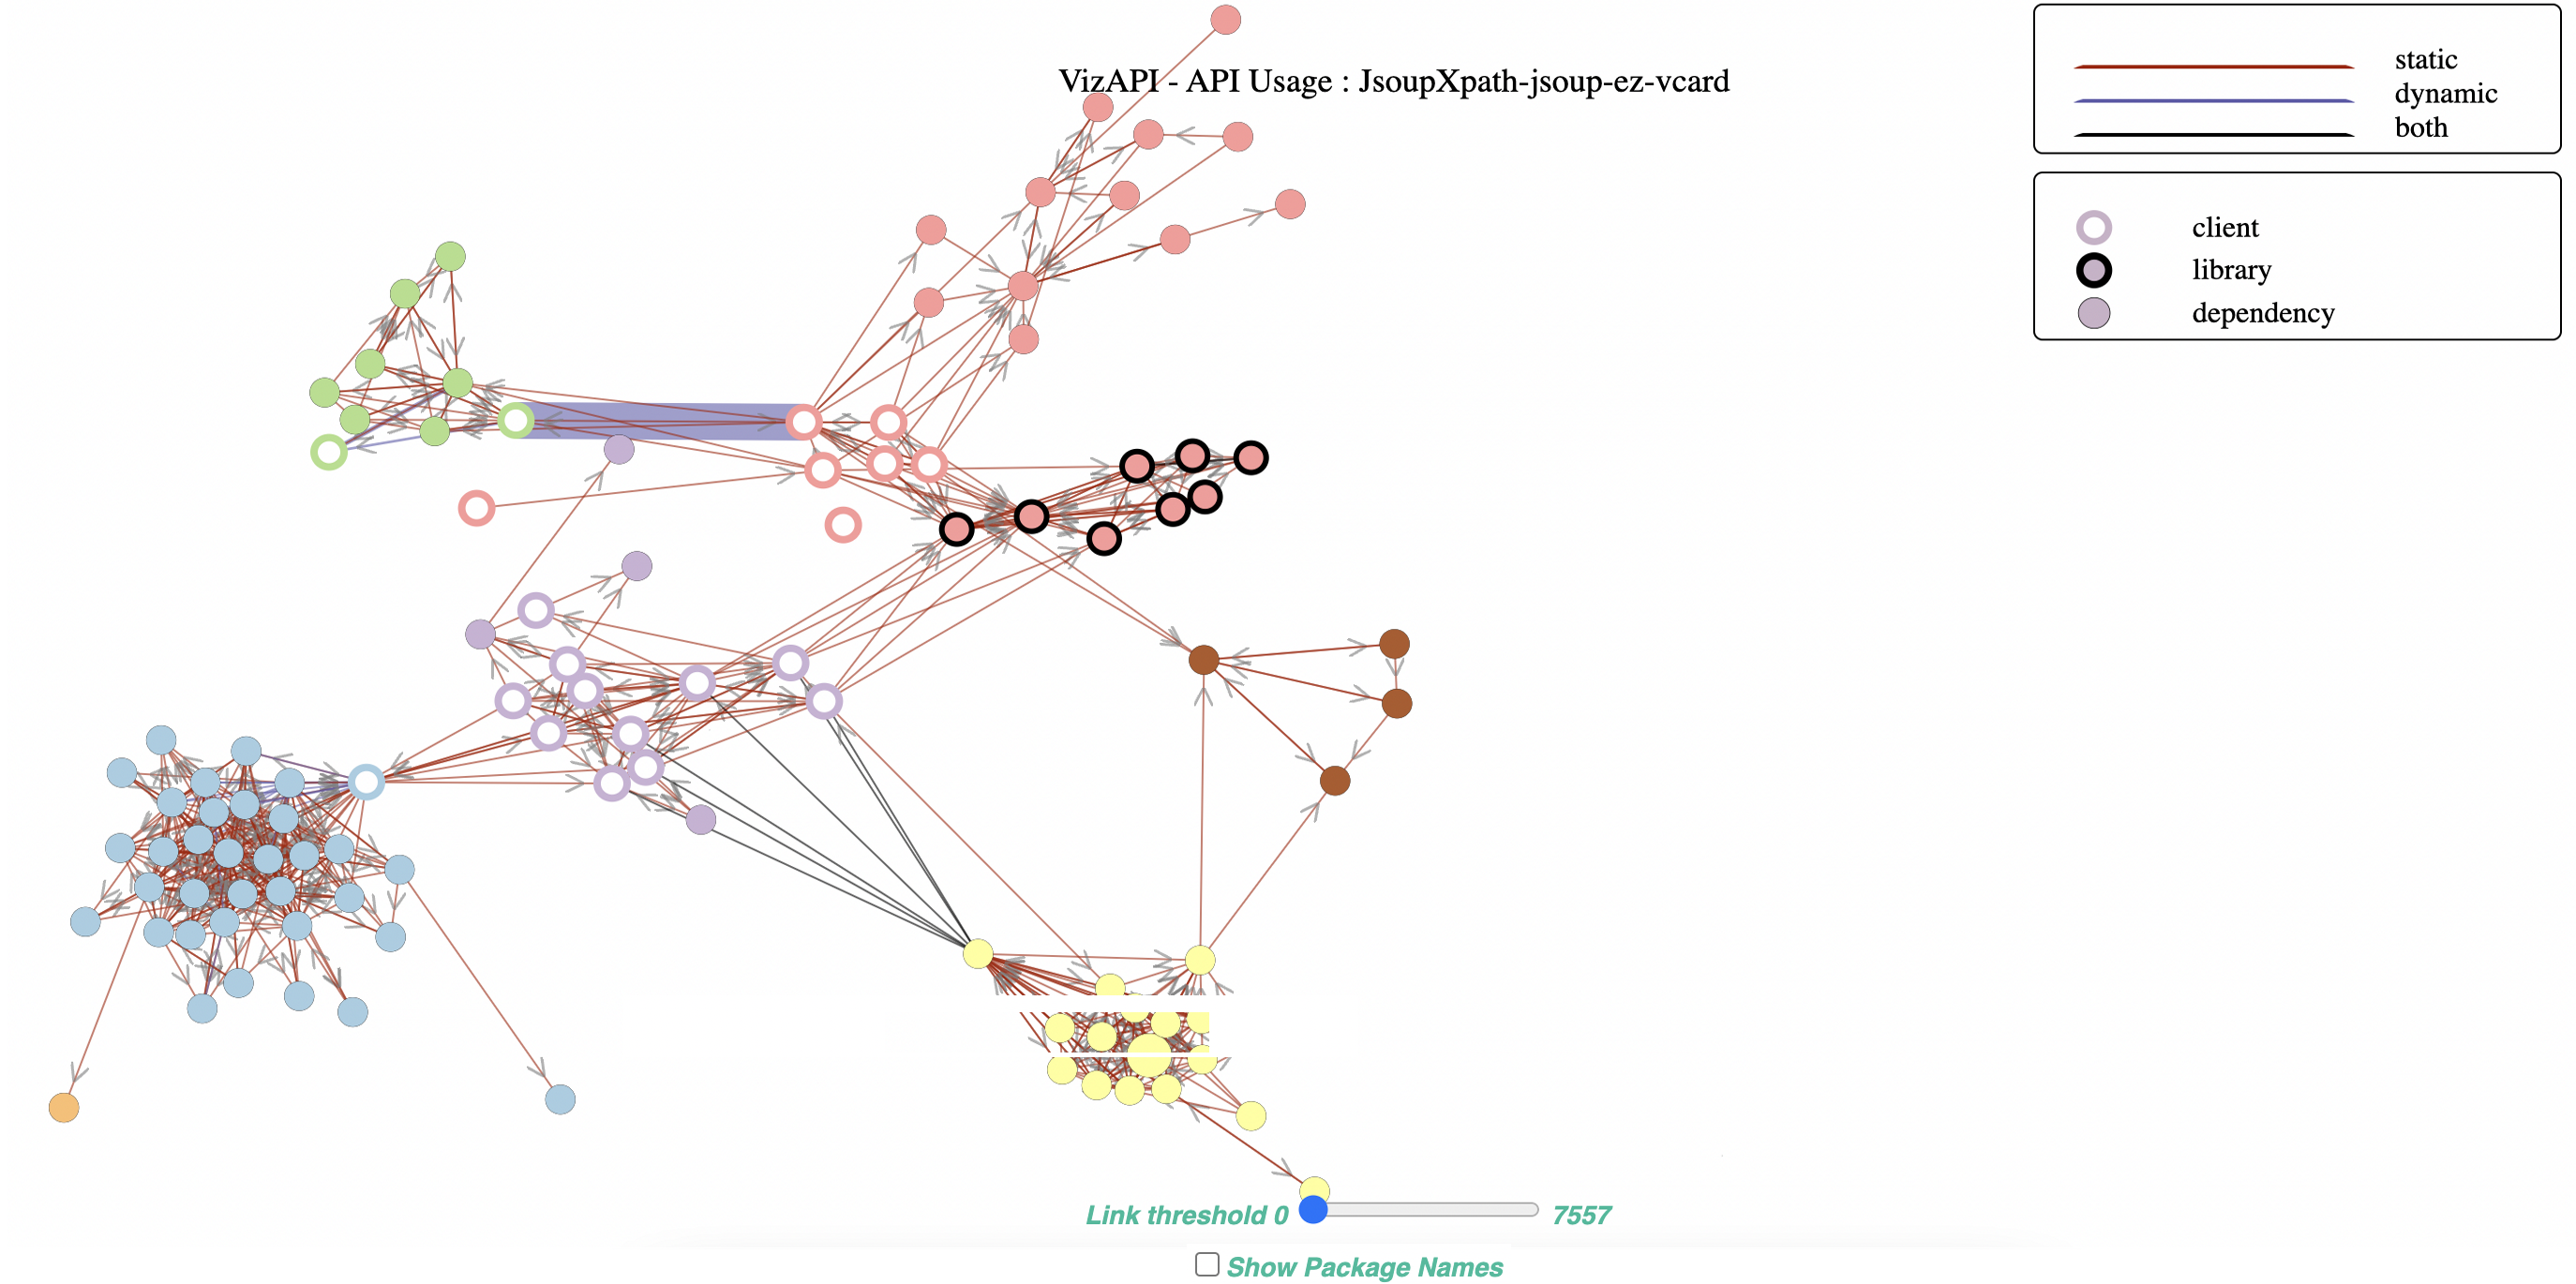
\includegraphics[width=16cm]{images/usage-scenario1.pdf}}
\hspace{7mm}

\subfloat[Usage Scenario 2: Client \textit{dataprocessor} (hollow, orange border) calls only one package in library \textit{fastjson} (green fill).
\label{fig:usagescenario2}]
{
\makebox[16cm]{
\includegraphics[width=11cm]{images/usage-scenario2.pdf}
}
}
\caption{\label{fig:usagescenarios} VizAPI Usage Scenarios.}

\end{center}
\end{figure*}


Once we have generated data from our tool that runs the static and dynamic analyses, we use a modified version
of the d3graph\footnote{\url{https://pypi.org/project/d3graph/}} library in Python to generate a d3js\footnote{\url{https://d3js.org/}}
visualization. The modifications that we made to the d3graph  library in Python in Python include multiple styling changes (for example, changing node styles based on whether it is a client, library or dependency),
legends and a toggle to show all package names. 
The graphs in Figures~\ref{fig:example}, \ref{fig:usagescenario1} and \ref{fig:usagescenario2} are examples of graphs produced by VizAPI.

VizAPI graphs are force-directed graphs based on the frequency of
interactions between different software components.  Each node is a
set of one or more packages that belong to the same JAR.  There are
three categories of nodes: clients are represented by nodes with white
interiors; libraries by nodes with filled interiors and black borders;
and dependencies (called by libraries but not clients) by nodes with
filled interiors and normal borders.  We coalesce nodes if they
originate from the same JAR and have the same incoming and
outgoing edges.

Each edge is directed
from the source package(s) to the target package(s) and represents an interaction 
(invocations, fields, annotations, subtyping) between packages. 
The thickness of each edge reflects the frequency of interactions between the source and the target.
Double-clicking on a node emphasizes its direct interactions with other packages while fading out the rest of the graph.

We run a Python implementation of the Louvain clustering algorithm~\cite{blondel2008fast}, and make the clusters 
visible by colouring nodes based on cluster.
This means that the same colour could indicate nodes (of the same category) from the same or different JARs.
Hovering on a node shows the list of packages and 
the JAR that they belong to, 
formatted as “jar : $\langle$space separated list of packages$\rangle$”. 

\subsection{Case Study}
\label{subsec:evaluation}

We conducted a pilot study of VizAPI.
We have generated data from our benchmarks.
We have collected both static and dynamic data for these projects, 
and we are in a position
to generate graphs for combinations of clients and libraries
in these projects. 
We present two usage scenarios below; graphs for 
our usage scenarios are publicly available.\footnote{\url{https://sruthivenkat.github.io/VizAPI-graph/}}
We intend for these usage scenarios to show how VizAPI can be useful to client developers when they want to observe library API usage and for library developers when they want to observe how their library is used by clients.

\paragraph{Usage Scenario 1: jsoup}
Imagine that we are a jsoup developer and want to understand
how some clients interact with it, in anticipation of making some breaking changes. We choose clients JsoupXpath\footnote{\url{https://github.com/zhegexiaohuozi/JsoupXpath}\label{jsoupxpath}} and ez-vcard\footnote{\url{https://github.com/mangstadt/ez-vcard}\label{ez-vcard}}.
Figure~\ref{fig:usagescenario1} shows static and dynamic interactions of the 2 clients with the jsoup\footnote{\url{https://github.com/jhy/jsoup}\label{jsoup}} library. Recall that nodes represent packages and edges represent interactions (usually invocations) between packages. 

We can start our exploration with the cluster of pink nodes. Many of these nodes belong to either JsoupXpath or jsoup. Hovering over a node tells us the package names while double-clicking shows us its direct interactions. (To search for a package, we can click on ``show package names'' and use the browser's find functionality.) Here, client JsoupXpath calls directly into \texttt{org.jsoup.nodes} and \texttt{org.jsoup.select}. Notably, and as we might expect, we can see that \texttt{org.jsoup.helper} and \texttt{org.jsoup.internal} aren't called directly by JsoupXpath. This would mean that breaking changes in \texttt{org.jsoup.helper} or \texttt{org.jsoup.internal} wouldn't directly affect JsoupXpath\footnote{As a specific example, the retraction of an internal jsoup API would not break this client. Behavioural changes that are directly passed through to the external API, for example, through delegation, can still break clients, but we can consider those to be changes in the external API.} 

Similarly, ez-vcard, which belongs to the purple cluster in Figure~\ref{fig:usagescenario1}, directly calls into \texttt{org.jsoup}. ez-vcard also calls into jackson-core\footnote{\url{https://github.com/FasterXML/jackson-core}\label{jackson-core}} and jackson-databind\footnote{\url{https://github.com/FasterXML/jackson-databind}\label{jackson-databind}}, which are very tightly coupled amongst their own packages and with each other. As a jsoup developer, we would be indifferent since it does not affect us; others, however, can observe that breaking changes in jackson-core and jackson-databind could propagate.

\paragraph{Usage Scenario 2: dataprocessor}

Figure~\ref{fig:usagescenario2} presents a second usage scenario. Here, say we are the developers of client dataprocessor\footnote{\url{https://github.com/dadiyang/dataprocessor}\label{dataprocessor}} (hollow with orange border). This client uses the fastjson\footnote{\url{https://github.com/alibaba/fastjson}\label{fastjson}} library (green fill). Our visualization shows calls only from dataprocessor package \texttt{com.github.dataprocessor.slice}, which is the orange-bordered client node (identity of the package available by hovering) to the package \texttt{com.alibaba.fastjson}. No other parts of dataprocessor use fastjson. This means that when we, as dataprocessor developers, need to upgrade the fastjson version, we only need to inspect the source code in our \texttt{com.github.dataprocessor.slice} package and cross-reference against release notes for fastjson. 

Note also the disconnected nodes in Figure~\ref{fig:usagescenario2}. These are all packages of fastjson that are not used by dataprocessor: any breaking changes in these packages definitely do not directly affect dataprocessor, and are less likely to affect it overall than packages that are directly used.

\section{Library Fission}
Modern software extensively reuses existing functionality using third-party libraries. Over time, libraries tend to extend their functionality, introducing more features and modifying existing ones. This leads to huge library sizes, a lot of which goes unused by a client that imports it. We have observed that modern API surfaces are vast and include thousands of potential access points, of which only hundreds are used by any typical client.This is called software bloating and there has been work around debloating. Debloating focuses on a single client at a time; it depends on dynamic analysis based on the client’s execution. We instead propose library fission, which focuses on splitting libraries based on client usage. This is a more permanent solution to bloating and does not require running analyses on clients for every execution. (We aim to split libraries based on client behaviour in a way that sub-modules of the fissioned library have common functionality.)

We use the data generated by our static and dynamic analyses to experiment with fissioning a subset of our corpus of libraries. On a high level, by library fission, we mean that we separate packages of a library into different Maven submodules. The following are the steps we follow to perform library fission for a given library, $L$:
\begin{enumerate}
\item Filter out all interactions with $L$, i.e., client uses of $L$, $L$'s uses of dependencies and intra-library uses of $L$.
\item Run the Louvain clustering algorithm on the filtered data where each node is set to be a package belonging to a jar.
\item Split up $L$ into Maven submodules based on the clusters.
\item Test on a subset of $L$'s clients.
\end{enumerate}

We now discuss specific examples from our libraries.

\subsection{\emph{fastjson}}
\label{sec:fastjson-fission}

We have 26 clients for \emph{fastjson}. Based on the usages of these clients, we obtained the following initial set of 5 clusters:
\begin{itemize}
\item Cluster 1:
\begin{itemize}
\item \texttt{com.alibaba.fastjson.annotation}
\item \texttt{com.alibaba.fastjson.asm}
\item \texttt{com.alibaba.fastjson.parser}
\item \texttt{com.alibaba.fastjson.serializer}
\item \texttt{com.alibaba.fastjson.support.hsf}
\item \texttt{com.alibaba.fastjson.support.config}
\item \texttt{com.alibaba.fastjson.support.retrofit}
\item \texttt{com.alibaba.fastjson.support.springfox}
\end{itemize}
\item Cluster 2:
\begin{itemize}
\item \texttt{com.alibaba.fastjson}
\end{itemize}
\item Cluster 3:
\begin{itemize}
\item \texttt{com.alibaba.fastjson.util}
\item \texttt{com.alibaba.fastjson.parser.deserializer}
\end{itemize}
\item Cluster 4:
\begin{itemize}
\item \texttt{com.alibaba.fastjson.support.spring}
\item \texttt{com.alibaba.fastjson.support.spring.annotation}
\end{itemize}
\item Cluster 5:
\begin{itemize}
\item \texttt{com.alibaba.fastjson.support.jaxrs}
\end{itemize}
\end{itemize}

We observe that the clusters are loosely based on functionality, that is, the packages within a cluster have similar functionality. This is not strictly true for all packages, but it is a good approximation. We see that the \texttt{jaxrs} and \texttt{spring} functionalities are clusters of their own and it makes sense to separate these into submodules since they provide their own independent functionality. However, we observed that there exist cyclic dependencies between Cluster 1, 2 and 3. If a library developer performs library fission and they run into cyclic dependencies, we recommend that they resolve these dependencies by moving classes into appropriate submodules. Due to our lack of domain knowledge (we don't know about what individual \emph{fastjson} classes do), we combined these 3 clusters into one submodule. Our final submodules are as follows:
\begin{itemize}
\item Submodule 1 --- utils:
\begin{itemize}
\item \texttt{com.alibaba.fastjson.annotation}
\item \texttt{com.alibaba.fastjson.asm}
\item \texttt{com.alibaba.fastjson.parser}
\item \texttt{com.alibaba.fastjson.serializer}
\item \texttt{com.alibaba.fastjson.support.hsf}
\item \texttt{com.alibaba.fastjson.support.config}
\item \texttt{com.alibaba.fastjson.support.retrofit}
\item \texttt{com.alibaba.fastjson.support.springfox}
\item \texttt{com.alibaba.fastjson}
\item \texttt{com.alibaba.fastjson.util}
\item \texttt{com.alibaba.fastjson.parser.deserializer}
\end{itemize}
\item Submodule 2 --- spring:
\begin{itemize}
\item \texttt{com.alibaba.fastjson.support.spring}
\item \texttt{com.alibaba.fastjson.support.spring.annotation}
\end{itemize}
\item Submodule 3 --- jaxrs:
\begin{itemize}
\item \texttt{com.alibaba.fastjson.support.jaxrs}
\end{itemize}
\end{itemize}

When we split \emph{fastjson} into submodules, we observed that each submodule needed fewer dependencies in the pom compared to the current version of \emph{fastjson} that is not split. The current version of \emph{fastjson} has 61 dependencies, while \emph{utils} has 47, \emph{spring} has 27 and \emph{jaxrs} has 29. Importing one of these newer submodules means a smaller probability of propagated vulnerabilities, version conflicts and breaking changes.

We sent an email to the \emph{fastjson} contributors proposing a split and did not receive a response, after which we created a pull request\footnote{\url{}https://github.com/alibaba/fastjson/pull/4276}. Our PR text was as follows:
``This PR splits fastjson into 3 submodules - utils, spring, jaxrs. We're looking into Java API usage as part of research and propose this split. These submodules are based on usage patterns that we've observed clients making of fastjson. It is beneficial to clients – they can import only the submodule they need to use (utils seems to be most popular). After this change, clients will not be affected by breaking changes in unused submodules and can avoid version conflicts and vulnerabilities propagated through dependencies. We believe that this split makes it easier to release backward compatible versions of fastjson and to isolate breaking changes."

\subsection{\emph{jsoup}}
\label{sec:jsoup-fission}

Based on usage by the 7 clients of jsoup we have in our benchmark set, we observed the following clusters:
\begin{itemize}
\item Cluster 1:
\begin{itemize}
\item \texttt{org.jsoup.parser}
\item \texttt{org.jsoup.safety}
\item \texttt{org.jsoup.helper}
\item \texttt{org.jsoup.internal}
\end{itemize}
\item Cluster 2:
\begin{itemize}
\item \texttt{org.jsoup}
\item \texttt{org.jsoup.examples}
\end{itemize}
\item Cluster 3:
\begin{itemize}
\item \texttt{org.jsoup.select}
\item \texttt{org.jsoup.nodes}
\end{itemize}
\end{itemize}

We observed multiple cyclic dependencies. In the case of cyclic dependencies, it is best for the library developers to split classes in packages and move them to clusters based on functionality. 

We now discuss a few interesting things we noted in the \emph{jsoup} clusters. Cluster 1 contains \texttt{org.jsoup.internal}. It is clear from the naming that this package is meant for internal use only and not for clients. We suggest that such packages be moved to a separate submodule so that clients are not tempted to import them. Similarly, Cluster 2 contains \texttt{org.jsoup.examples} which also almost certainly will not be needed by clients and can also be moved to a separate submodule. 

Due to the multiple cyclic dependencies that we observed, we did not raise a pull request for \emph{jsoup}.

\section{Upgrades, Breaking Changes and Backward Compatibility}
Our data for 101 Java software components contains different kind of interactions across component boundaries. This data can be analyzed and prove useful in the following ways:
\begin{itemize}
\item Library developers can observe different usage patterns of their APIs. The clusters observed in library packages can help with new version releases. Breaking changes might be restricted to clusters and library developers can choose whether to make clusters from new versions backward compatible with other clusters from older versions or not. 
\item Clients can also check if breaking changes in new library versions will affect their code during upgrades and cross check this with library changelogs. 
\item Unused dependencies can be identified and removed to prevent them from possibly introducing version conflicts and vulnerabilties.
\end{itemize}